

\subsection{Developer Validation}
\label{subsec.opencard}

To further validate the influential software changes dataset that we have
collected with our intuition-based post-mortem metrics, we perform a large-scale developer study. Instead of asking developers to confirm each identified
commit, we must summarize the commits into categories. To that end, we
resorted to open-card sorting~\cite{Nielsen95}, a well known, reliable and
user-centered method for building a taxonomy of a system~\cite{boxesandarrows}.
Card sorting helps explore patterns on how users would expect to find content
or functionality. In our case, we use this technique to label influential
software changes within categories that are easily differentiable for
developers.

We consider open-card sorting where participants are given cards showing
description of identified influential software changes\footnote{We consider
all 177 influential software changes from the post-mortem analysis.} without
any pre-established groupings. They are then asked to sort cards into groups
that they feel are acceptable and then describe each group. We performed this
experiment in several iterations: 
\begin{itemize}
	\item first, two authors of this paper provided individually their group descriptions, based on the 177 influential changes identified from the post-mortem analysis.
	\item  second, the two authors then met to perform another open-card sorting with cards containing their agreed group descriptions. Table~\ref{tab:cards} enumerates the 28 cards that were then summarized.
	\item Finally, a third author, with more experience in open-card sorting, joined for a final group open-card sorting process which yielded 12 categories of influential software changes reported in Table~\ref{tab:ics}
\end{itemize}
 
\begin{landscape}
  
 \begin{table}
 \centering
 \scriptsize
 	\begin{tabular}{l|r}
 	\bf Card description & \bf Example commit description (only when not summary needs explanation) \\
 	\hline
 	\hline
 		Implementation of a long-awaited feature & \\ \hline
 		Change which was discussed at length as solving a bug that was very hard to reproduce &	\\ \hline
 		trivial fixes that has high impact on basic requirements for system functionality & (e.g., in commons-compress, simple fixes but it can prevent filepath encoding problems)	\\ \hline
 		Bug fix of a key feature in library & \\ \hline
 		\multirow{2}{*}{Bug fix of a bug that manifests itself only in corner-cases} & (e.g., This fix prevents data integrity violations, which cannot be revealed unless accessing missing data.)\\
 		& Bug fix to prevent an infinite loop when API reading input stream encounters an unmappable character \\
 		\hline
 		Replacement of key functionality code to improve usability & \\ \hline
 		Fix for a regression error that is hard to reproduce and that & (e.g., the change is about exception handling (whether it should be 	caught in the program and which place). \\ 
 		occurs in specific, but popular, environment  &This is not easy to reproduce. It happens in Google App Engine and the previous version works correctly.) \\ \hline
 		Fix for an API bug - the API is used pervasively	 & \\\hline
		New feature that was discussed at length	 & \\\hline
 		New feature that implements as an API a functionality that developers 		&	\\
 		implement regularly in an ad-hoc manner in their own code & \\ \hline
		Non-functional bug fix for speciific popular API -- leads to debate & (e.g., This change fixes a performance bug which affects Android applications. This change leads \\
&  to a long 	debate	since people have different opinions on this issue. The repaired method is popular.)\\ \hline
Change reverting a bug fix to a key functionality & \\ \hline
Controversial change that is debated and then reverted &\\\hline
Fix for a bug that affects many clients/components/applications (i.e., core component) &\\\hline
Fix to a Blocking Bug & \\\hline
Fix for non-functional defect & (e.g., Performance defect --- adding multicores could not improve the performance.)	\\
New API implementation for future applications & \\\hline
Fix of dependency problems for compilation & \\\hline
Fix of configuration errors & (e.g., New build references in POM files and assembly references)	\\\hline 
Fix of a trivial bug, but which appears in several different components 		& https://github.com/wildfly/wildfly/commit/eea5d5fe34e9e7c67f076cae81fec6ebf06626af	 \\ \hline
-- leads to debate and verification of all source code & \\ 
\multirow{2}{*}{Fix a bug that is not easy to locate} & (e.g., Yes, this change releases the hang (not failing nor crashing)	\\ 
&  of a test case. A test case hang can block maven building. \\ \hline
Change that overhauls an important module/file & \\ \hline
Change that add test cases to avoid specific important functional bugs & \\ \hline
Changefor improvement of implementation by creation of new exception class& \\ \hline
Change in nightly process management& \\ \hline
Bug fix that finalizes/corrects previous fix in API& \\ \hline
Changes that lead to several collateral changes (including reverting, new API mapping)& \\ \hline
 	\end{tabular}
 	\caption{Cards after the second-round of open-card sorting}
 	\label{tab:cards}
 \end{table}
 
 \end{landscape}
 
 
\begin{table} [!h]
\scriptsize
	\begin{tabular} {l | c | r}
	 {\bf Consensus-based label} & {\bf Description of influence} & {\bf Example change}\\ \hline 
	New key feature & \multicolumn{1}{p{4cm}|}{Implementation of a long awaited feature, change that implements as an API a functionality that developers implement regularly in an ad-hoc manner in their own code} & \multicolumn{1}{p{5.5cm}}{Implementation of the Kalman filter in the Commons-MATH project was tagged in {\tiny \url{https://issues.apache.org/jira/browse/MATH-485}} as a major feature request which was resolved by the change commit \url{https://github.com/apache/commons-math/commit/58d18852} }\\ \hline
	Domino Changes & \multicolumn{1}{p{4cm}|}{Change causing many collateral changes (e.g., change all API method call sites to reflect API modification)} & \multicolumn{1}{p{5.5cm}}{Starting with Linux 2.5.4, the USB library function usb\_submit\_urb (which implements message passing) now takes a second argument for explicitly specifying the context (which was previously inferred in the function definition). The argument can take one of three values: GFP\_KERNEL (no constraints), GFP\_ATOMIC (blocking is not allowed), or GFP\_NOIO (blocking is allowed but not I/O)). Developers using this USB library must then parse their own code to understand which context it should be. This leads to bugs that can keep occurring. A study of faults in Linux by Pallix et al.~\cite{Palix10Faults} have reported that, due to the complexity of the conditions governing the choice of the new argument for usb submit urb, 71 of the 158 calls to this function were initially transformed incorrectly to use GFP KERNEL instead of GFP\_ATOMIC.}\\ \hline
	API Usability Improvement &\multicolumn{1}{p{4cm}|}{Replacement of key functionality code to improve usability, or introduction of new error management (e.g., improvement of implementation by creation of a new exception class, or log management for users)} & \multicolumn{1}{p{5.5cm}}{In the Wildfly project, a major feature request ({\tiny \url{https://issues.jboss.org/browse/WFLY-280}}) was resolved for providing an operation to retrieve the last 10 errors from the log. Discussions on the issue page clearly shows that the change was solving a major issue as it improved usability substantially ({\tiny \url{https://github.com/wildfly/wildfly/commit/a22b8d7ccf872b503da8d43f1c29390356d6d5d3}}) }\\ \hline
	Major Structural Change & \multicolumn{1}{p{4cm}|}{Change that overhauls an important module/file} & \multicolumn{1}{p{5.5cm}}{Commit 34658f08 ({\tiny \url{https://github.com/apache/commons-lang/commit/34658f08}}) in the commons-LANG project rewrites an entire utils file }\\ \hline
	Fix configuration bug & \multicolumn{1}{p{4cm}|}{Fix of dependency problems for compilation, change in nightly build process management} & \multicolumn{1}{p{5.5cm}}{In the WILDFLY project a major bug (https://issues.jboss.org/browse/WFLY-2047) was finally resolved by fixing dependencies in the connector module ({\tiny \url{https://github.com/wildfly/wildfly/commit/88756ddb1061660cb5ca68f5562d7343570dd955}})}\\ \hline
	Important test case addition & \multicolumn{1}{p{4cm}|}{Changes that add test cases to avoid specific important functional bugs} & \multicolumn{1}{p{5.5cm}}{Commit 1f001d06 ({\tiny \url{https://github.com/apache/commons-lang/commit/1f001d06}}) in the LANG project specifically added some test cases to avoid regression faults on key functionalities.}\\ \hline
	Fix non-functional bug & \multicolumn{1}{p{4cm}|}{Non-functional bug fix for a specific API. Performance or security issues usually lead to debate among developers } & \multicolumn{1}{p{5.5cm}}{ A change in Commons-math project fixes a performance bug which affects Android applications ({\tiny \url{https://github.com/apache/commons-math/commit/52649fda4c9643afcc4f8cbf9f8527893fd129ba}}). This change leads to a long debate since people have different opinions on this issue. Although this does not affect the functionality of the method, the repaired method is popular}\\\hline
	Fix hard to reproduce/locate bug & \multicolumn{1}{p{4cm}|}{Fix of a bug that manifests itself only in corner-cases, or a bug that is not easy to locate, or a bug that is simply hard to reproduce} & \multicolumn{1}{p{5.5cm}}{A change in the Spring framework fixes a regression fault that is not easy to reproduce (cf. {\tiny \url{https://github.com/spring-projects/spring-framework/commit/956b66bbd466bb7a68e8499a483139a516572b24}}).}\\\hline
	
		\end{tabular}
	%\caption{List of 12 Influential Changes labeled during Open Card Sorting}
\end{table}

\begin{table}
\scriptsize
	\begin{tabular} {l | c | r}
	% {\bf Consensus-based label} & {\bf Description} & {\bf Example}\\ \hline 
	\hline
	Fix blocking bug & \multicolumn{1}{p{4cm}|}{Fix a bug that prevents other bugs from being exposed/addressed} & \multicolumn{1}{p{5.5cm}}{In project CASSANDRA, commit d37696ca provides a change that fixes partially a major blocking bug}\\ \hline
	Fix pervasive bug & \multicolumn{1}{p{4cm}|}{Fix of a bug that affects many clients/components/applications(i.e, core component),  fix a bug which may also appear in several different components, or  fix of an API that is used pervasively} & \multicolumn{1}{p{5.5cm}}{In the Spring framework, a change in the equality operator is pervasively affecting other components ({\tiny \url{https://github.com/spring-projects/spring-framework/commit/2a05e6afa116ab56378521b5e8c834ba92c25b85}}).}\\
	Fix key feature bug & \multicolumn{1}{p{4cm}|}{Bug fix of a key feature in library or fix that has high impact on basic requirements for system functionality}& \multicolumn{1}{p{5.5cm}}{In Commons-COMPRESS project, a bug fix change (fadbb4cc) was applied to fix the implementation of the zip functionality. Indeed, creating a zip file with many entries was producing a wrong archive}\\ \hline
	Correcting controversial change & \multicolumn{1}{p{4cm}|}{Bug fix that finalizes/corrects previous fix in API, change reverting a bug fix to a key functionality or controversial change that is debated and then reverted} &  \multicolumn{1}{p{5.5cm}}{changes in the Spring Framework ({\tiny \url{https://github.com/spring-projects/spring-framework/commit/cfc821d1799ca7c64b1bbc53811b712fdaa4776c}} and  {\tiny \url{https://github.com/spring-projects/spring-framework/commit/0934751d7aa625fd098086ce3a5fb489f2edc7e0}}) are fixing regression faults that could not be easily reproduced. These changes were reverted several times due to incomplete fixes}\\ \hline \hline
		
	\end{tabular}
	\caption{List of 12 Influential Changes labeled during Open Card Sorting, with examples of changes in these categories}
	\label{tab:ics}
\end{table}


The influential software changes described in the 12 categories span over
four software maintenance categories initially defined by Lientz {\em et
al.}~\cite{Lientz:1978:CAS:359511.359522} and updated in ISO/IEC 14764. Most
influential software changes belong to the {\em corrective changes} category.
Others are either {\em preventive changes}, {\em
adaptive changes} or {\em perfective changes}. Finally, changes in one of our influential change categories
 can fall into more than one maintenance categories. We refer to
them as {\em cross area changes}.



\textbf{Developer assessment.}
We then conduct a developer survey to assess the relevance of the 12 categories of influential changes that we describe. 
The survey participants have been selected from data collected in the GHTorrent project~\cite{Gousi13} which contains history
archives on user activities and repository changes in GitHub. We consider active developers (i.e., those who have contributed in the latest changes recorded in GHTorrent) and focus on those who have submitted comments on other's commit. We consider this to be an indication of experience with code review. The study\footnote{Survey form at \url{https://goo.gl/V2g8OE}} was sent to over 1952 developer email addresses. After one week waiting period, only 800 email owners opened the mail and 144 of them visited the survey link. Finally 89 developers volunteered to participate in the survey. 66 (i.e., 74\%) of these developers hold a position in a software company or work in freelance. Nine respondents (10\%) are undergraduate students and eight (9\%) are researchers. The remaining six developers did not indicate their current situation. In total, 78\% of the participants confirmed having been involved in code review activities. 26 (29\%) developers have between one and five years experience in software development. 29 (33\%) developers have between five and ten years of experience. The remaining 34 (38\%) have over ten years of experience. 

In the survey questionnaire, developers were provided with the name of a category of influential software changes, its description and an illustrative example from our dataset (we provided the same example for each category to every participant). The participant was then requested to assess the relevance of this category of changes as influential software using a Likert scale between {\tt 1:very influential} and {\tt 5:unimportant}. Figure~\ref{fig:survey} summarizes the survey results. For more detailed description of the categories, we refer the reader to the project web site (see Section ``Availability'').

The survey results suggest that:
\begin{itemize}
	\item According to software developers with code review experience, all 12 categories are about important changes: 7 categories have an average agreement of 2 (i.e., Influential), the remaining 5 categories have an average of 3 (i.e., potentially influential). Some (e.g.,  ``domino changes'' and ``changes fixing pervasive bugs'') are clearly found as more influential than others (e.g., ``important test case addition'').
	\item Some changes, such as ``fixes for hard to reproduce or locate bugs'', are not as influential as one might think.
	\item Developers also suggested two other categories of influential changes: {\em Documentation changes} and {\em Design-phase changes}. The latter however are challenging to capture in source code repository artefacts, while the former are not relevant to our study which focuses on source code changes.
\end{itemize}

With this study we can increase our confidence in the dataset of influential
software changes that we have collected. We thus consider leveraging on the
code characteristics of these identified samples to identify more influential
changes.


%\begin{sidewaysfigure}[ht]


\begin{landscape}

 \begin{figure}
 \centering
\scriptsize
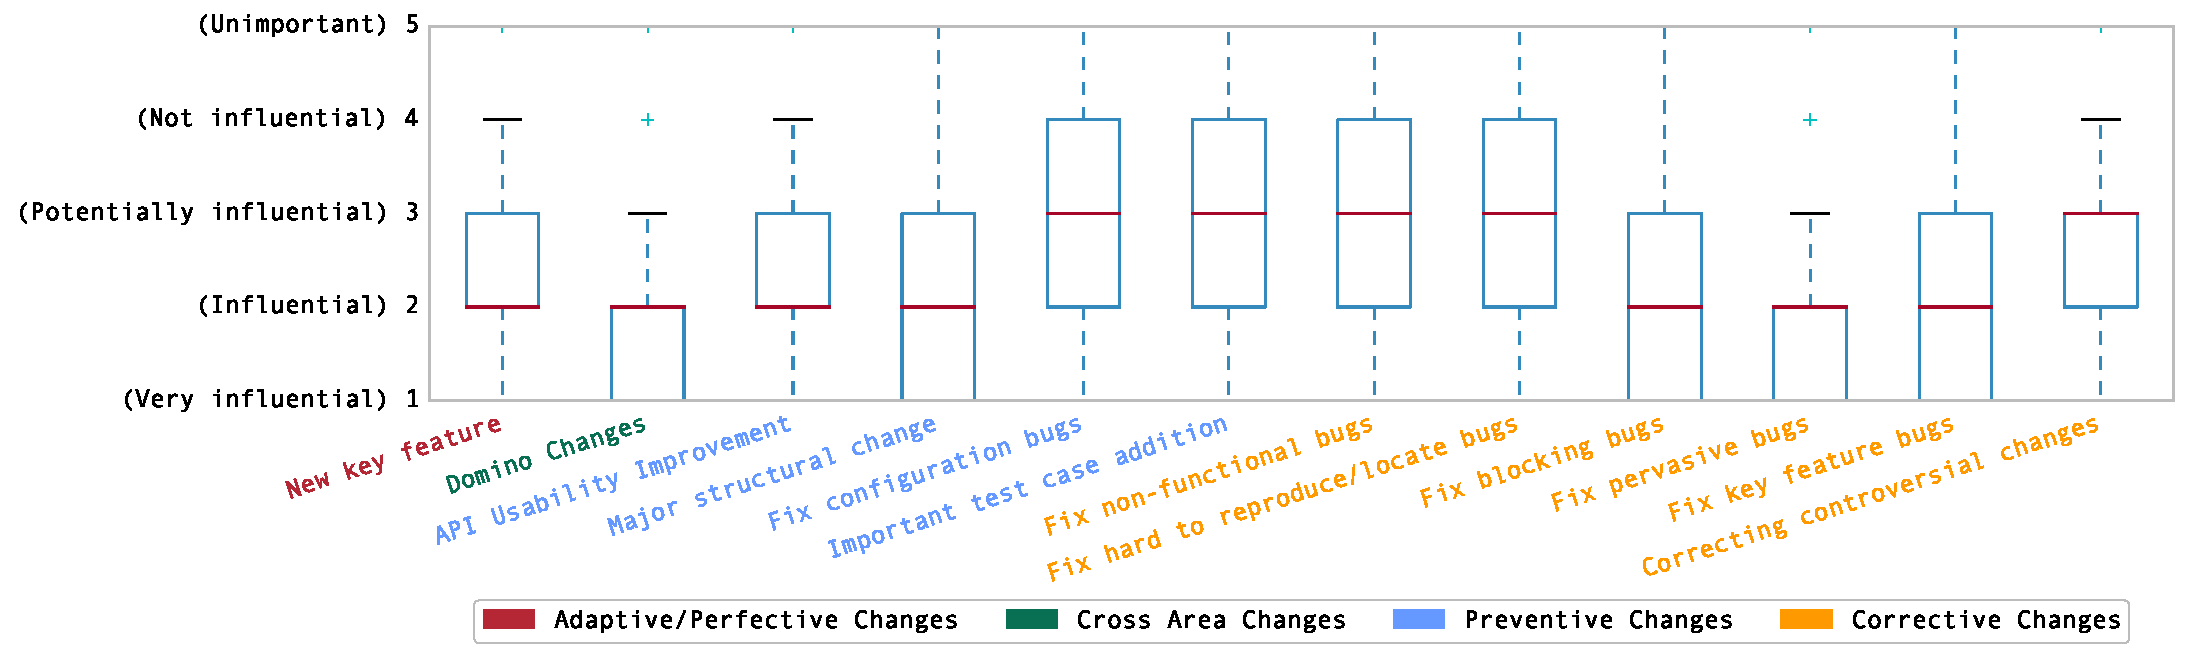
\includegraphics[width=\linewidth]{fig/response-boxplot.pdf}
\caption{Survey results on different categories of Influential Changes.}
\label{fig:survey}
%\end{sidewaysfigure}
 \end{figure}

\end{landscape}

